% !TeX program = lualatex
\documentclass[a5paper,11pt,openany]{article}
\usepackage{orcidlink}

\usepackage{blindtext}
%\usepackage[style]{abstract}

\usepackage[top=2cm,bottom=2cm,bindingoffset=0cm]{geometry}

\usepackage[svgnames]{xcolor} % Required to specify font color

%\documentclass[a4paper,12pt,openany]{scrbook}

%\usepackage{glossaries}
%\usepackage[xindy]{glossaries}
%\makeglossaries

%\usepackage{odsfile,lmodern}

%\usepackage{luacode}


\usepackage{multicol}

%\usepackage{churchslavonic}
%\usepackage{polyglossia}
%\setotherlanguages{russian,churchslavonic}

\usepackage{mathtext}
\usepackage{makeidx}
%\usepackage{imakeidx}
\usepackage{longtable}
\usepackage[tc]{titlepic}

\usepackage{fontspec}

\usepackage[protrusion=true,expansion,
tracking=true,letterspace=50]{microtype}


%\usepackage{academicons}
%\usepackage{xcolor}


%\SetTracking[ spacing = {25*,166, } ]{ encoding = *, shape = sc }{ 25 }


%\usepackage{soulutf8}
%\usepackage{letterspace}

%\usepackage[toc]{appendix}
\usepackage[toc,titletoc]{appendix}
\renewcommand\appendixtocname{Приложения}
\renewcommand\appendixpagename{Приложения}

%\usepackage{xunicode}
\usepackage{xltxtra}

\usepackage[normalem]{ulem}
\usepackage{adjustbox}

\usepackage{polyglossia}
\setmainlanguage{russian}
\setdefaultlanguage{russian}
\setotherlanguage{ukrainian}
\setotherlanguage{english}
\setotherlanguage{greek}
\setotherlanguage{latin}
\setotherlanguage{polish}


\setmainfont[BoldFont={DejaVuSerif-Bold.ttf},
ItalicFont={DejaVuSerif-Italic.ttf},
 BoldItalicFont={DejaVuSerif-BoldItalic.ttf}]{DejaVuSerif.ttf}

\setromanfont[BoldFont={DejaVuSerif-Bold.ttf},
ItalicFont={DejaVuSerif-Italic.ttf},
 BoldItalicFont={DejaVuSerif-BoldItalic.ttf}]{DejaVuSerif.ttf}

\setsansfont[BoldFont={DejaVuSans-Bold.ttf},
ItalicFont={DejaVuSans-Oblique.ttf},
 BoldItalicFont={DejaVuSans-Oblique.ttf}]
{DejaVuSans.ttf}

\setmonofont[BoldFont={DejaVuSansMono-Bold.ttf},
ItalicFont={DejaVuSansMono-Oblique.ttf},
 BoldItalicFont={DejaVuSansMono-BoldOblique.ttf}]
{DejaVuSansMono.ttf}



\usepackage{enumitem}
\usepackage{indentfirst} 

\usepackage{verse}

\usepackage{graphicx}

%\usepackage[pdfpagelabels,unicode,plainpages=false]{hyperref}

\hypersetup{pdftitle=Упыри в роду Гоголя. Петр Семилетов.}

\usepackage{bookmark} 
\usepackage{relsize}

\usepackage{tocloft,calc}
\usepackage[nottoc,numbib]{tocbibind}


\frenchspacing
\righthyphenmin=2


\makeatletter
\@addtoreset{chapter}{part}
\makeatother  


%\titlepic{\includegraphics[width=0.50\textwidth]{cover/04.jpg}}

\title{УПЫРИ В РОДУ ГОГОЛЯ\\
\textsmaller[2]{редакция 1.0}}
\author{Петр Семилетов\\ORCID:0009-0002-3901-7785 \orcidlink{0009-0002-3901-7785}}
\date{26/03/2025}



\newcommand*{\plogo}{\fbox{$\mathcal{PL}$}} % Generic publisher logo

% –  –  –  –  –  –  –  –  –  –  –  –  –  –  –  –  –  –  –  –  –  –  –  –  –  –  –  –  –  –  –  –  –  –  –  –  –  –  –  –  –  –  –  – 


\begin{document}


\maketitle

\pagestyle{empty}


\newpage

\pagestyle{plain}

%\hrule

%\tableofcontents

%\input{pre/pre.tex}
%\input{plan-right/plan-right.tex}
%\input{plan-right/plan-right-text.tex}

\begin{abstract}
Работа посвящена вопросу о том, что Гоголя похоронили живым, а также родне Гоголя, среди которой находим людей, прослывших упырями.
\end{abstract}


\section{Кто такие упыри}

   Услышав слово вампир, вы представляете себе бледного человека в черном плаще, который скалит острые клыки. Он спит в гробу, и имеет ряд дурных привычек, вроде лазания по стенам, превращения в летучую мышь и конечно же напиткам предпочитает кроооовь. Таков образ вампира в книгах, играх и кино.

   В народных же представлениях вампиры, а у восточных славян упыри или опыри – явление совсем иного рода. Это люди, которые родились ведьмачами, колдунами. В народе считалось, что ведьмачи бывают прирожденные и «ученые», то бишь наученные. Так вот упыри это первые. Кроме прочего, они могут впадать в состояние, можно сказать, глубокого транса, когда нельзя распознать ни дыхание, ни биение сердца. 

   Кстати, Снорри Стурлусон в «Круге земном», собрании преданий Исландцев, пишет сходное о скандинавском боге Одине. Один ведь был смертным человеком, его обожествили посмертно. И вот что написано про Одина:

\begin{quotation}
\noindent Один мог менять свое обличье. Тогда его тело лежало, как будто он спал или умер, а в
это время он был птицей или зверем, рыбой
или змеей и в одно мгновение переносился в
далекие страны по своим делам или по делам
других людей.
\end{quotation}

Это описание оборотничества, не киношного, но с переключением сознания от одного тела к другому. 

И когда человек находился в этом странном состоянии, его вполне могли счесть мертвым и похоронить. Подобные люди приходили в себя в могиле, пытались выбраться, и некоторым это удавалось. Чем это для них заканчивалось, известно – осиновым колом в грудь. Кое-где считали, что телом такого покойника управляет уже не его душа, но вселившийся бес. 

   Как бы ни было, думаю так возникло представление, что колдуны-упыри после смерти оживают и начинают вредить людям.

   Упырями или одминами, то бишь подменышами, называли также детей, как считали собиратели фольклора, «больных рахитом». У них было, согласно описаниям, размягчение костей, большие головы, длинные тонкие ноги. Эти дети не могли ходить, зато имели дар ясновидения, и рано умирали. Про них после смерти плохие слухи не множились, но была молва, что такие упыри сразу после смерти снова рождаются в другом, подобном теле, и опять дают предсказания. Любопытные отголоски прежних верований в христианской среде.


\section{Гоголь}

Николай Гоголь в вышедшей в начале 1847 года книге «Выбранные места из переписки с друзьями» в начале поместил не письмо, но своё завещание, вероятно полагая, что первые страницы прочтут наверняка и примут к сведению. Вот отрывок сего документа:

\begin{quotation}
\noindent I. Завещаю тела моего не погребать до тех пор, пока не покажутся явные признаки разложения. Упоминаю об этом потому, что уже во время самой болезни находили на меня минуты жизненного онемения, сердце и пульс переставали биться… Будучи в жизни своей свидетелем многих печальных событий от нашей неразумной торопливости во всех делах, даже и в таком, как погребение, я возвещаю это здесь в самом начале моего завещания, в надежде, что, может быть, посмертный голос мой напомнит вообще об осмотрительности.
\end{quotation}

Николая Васильевича Гоголя сочли мертвым в 8 часов утра 21 февраля 1852 года. Вскрытие не проводилось. Написали, что умер от простуды. Завещание не выполнили. Похоронили на погосте Данилова монастыря в Москве.

В 1931 году, в связи с преобразованием помещений монастыря в приёмник-распределитель для беспризорников и несовершеннолетних правонарушителей, кладбище решили уничтожить, перенеся однако ряд важных могил. Среди них оказалась могила Гоголя.

31 мая 1931 года была произведена эксгумация тела, во время которой присутствовали, кроме прочего, писатели Всеволод Иванов, Владимир Луговской, Михаил Светлов, Юрий Олеша, Владимир Лидин, историк Мария Барановская. Лидин позже делился увиденным, причем свидетельства в разное время разнились, но кажется именно слова Лидина породили слух, что Гоголя похоронили живым.

Досадную, содержащую оценочные суждения запись можно прочитать в Википедии: 

\begin{quotation}
Официальный акт экспертизы, составленный сотрудниками НКВД и ныне хранящийся в РГАЛИ (ф. 139, № 61), оспаривает малодостоверные и взаимоисключающие друг друга воспоминания участника и свидетеля эксгумации писателя Владимира Лидина.
\end{quotation}

Помещаю фотографию акта в разделе Иллюстраций, давайте почитаем его текст. Документ РГАЛИ «ф.139 оп.1 ед. хр.61 Акт о вскрытии могилы Н. В. Гоголя на кладбище бывшего Даниловского монастыря для погребения праха на Ново-Девичьем кладбище в г. Москве 31 мая 1931»:

\begin{quotation}
Акт

31-го мая 1931 года мы, нижеподписавшиеся, составили настоящий акт в том, что в нашем присутствии на кладбище бывш. Даниловского м-ря произведена эксгумация писателя Николая Васильевича Гоголя для перепогребения на новом кладбище бывш. Ново-Девичьего монастыря в Москве

подписи
\end{quotation}

И всё. Ничего более на бумажке нет. Каким образом сие оспаривает сведения Владимира Лидина, надо спросить у того, кто писал в Википедии.

Бывший студент Лидина, старший научный сотрудник Государственного Литературного музея Юрий Владимирович Алехин вспоминал: 

\begin{quotation}
У могилы он (Лидин) встретил собратьев по перу Вс. Иванова, В. Луговского, М. Светлова, Ю. Олешу. Их также оповестили накануне. Не обошлось и без людей из богемы, Бог весть как прознавших о перенесении праха. В большем числе явились комсомольцы из Хамовников (директор Новодевичьего кладбища был выдвинут от комсомола). Было несколько милиционеров.

Священников и убеленных сединой профессоров, что приличествовало бы событию, Лидин не увидел. Всего собралось 20−30 человек. 

Гроб понесли не сразу, вспоминал Лидин, он оказался почему-то не там, где копали, а несколько поодаль в стороне. А когда его извлекли из-под земли, с виду крепкий, из дубовых досок, и вскрыли, то к сердечному трепету примешалось еще… недоумение. В гробу лежал скелет с повернутым набок черепом. 

Объяснения этому никто не находил. Кому-нибудь суеверному, наверное, тогда подумалось: «Вот ведь мытарь — при жизни будто не живой и после смерти не мертвый, этот странный великий человек». 
\end{quotation}

В записке же самого Лидина относительно этих событий говорится иное:

\begin{quotation}
В июне 1931 года мне позвонил по телефону один из сотрудников Исторического музея.
«Завтра на кладбище Данилова монастыря будет происходить вскрытие могилы Гоголя, — сказал он мне. — Приезжайте».

Я поехал. Был тёплый летний день. По привычке я захватил с собой фотоаппарат. Снимки, которые я сделал на кладбище, оказались единственными. Одновременно с могилой Гоголя вскрыли в этот день могилы Хомякова и Языкова; прах их тоже подлежал перенесению. Кладбище Данилова монастыря упразднялось. На территории монастыря был организован приёмник для несовершеннолетних правонарушителей.

Могилу Гоголя вскрывали почти целый день. Она оказалась на значительно большей глубине, чем обычные захоронения. Начав её раскапывать, натолкнулись на кирпичный склеп необычайной прочности, но замурованного отверстия в нём не обнаружили; тогда стали раскапывать в поперечном направлении с таким расчетом, чтобы раскопка приходилась на восток (т. е., именно головой к востоку, по православному обряду, должен был быть предан земле покойник), и только к вечеру был обнаружен еще боковой придел склепа, через который в основной склеп и был в своё время вдвинут гроб.

Работа по вскрытию склепа затянулась, и начинались уже сумерки, когда могила была, наконец, вскрыта. Верхние доски гроба прогнили, но боковые с сохранившейся фольгой, металлическими углами и ручками и частично уцелевшим голубовато-лиловым позументом, были целы.

Вот что представлял собой прах Гоголя:
черепа в гробу не оказалось, и останки Гоголя начинались с шейных позвонков: весь остов скелета был заключён в хорошо сохранившийся сюртук табачного цвета; под сюртуком уцелело даже бельё с костяными пуговицами; на ногах были башмаки, тоже полностью сохранившиеся; только дратва, соединяющая подошву с верхом, прогнила на носках, и кожа несколько завернулась кверху, обнажая кости стопы. Башмаки были на очень высоких каблуках, приблизительно 4-5 сантиметров, это даёт безусловное основание предполагать, что Гоголь был невысокого роста.

Когда и при каких обстоятельствах исчез череп Гоголя, остаётся загадкой. При начале вскрытия могилы, на малой глубине, значительно выше склепа с замурованным гробом, был обнаружен череп, но археологи признали его принадлежавшим молодому человеку.

Прах Языкова и Хомякова мне удалось сфотографировать; останков Гоголя я, к сожалению, снять не смог, так как были уже сумерки, а на следующее утро они были перевезены на кладбище Новодевичьего монастыря, где и преданы земле. 

Я позволил себе взять кусок сюртука Гоголя, который впоследствии искусный переплётчик вделал в футляр первого издания «Мёртвых душ»; книга в футляре с этой реликвией находится в моей библиотеке.

Мне пришлось впоследствии слышать такую легенду: в 1909 г., когда при установке памятника Гоголю на Пречистенском бульваре в Москве, производилась реставрация могилы Гоголя, Бахрушин подговорил будто бы монахов Данилова монастыря добыть для него череп Гоголя и что, действительно, в Бахрушинском театральном музее в Москве имеются три неизвестно кому принадлежащие черепа: один из них по предположению — череп Щепкина, другой — Гоголя, о третьем ничего не известно. Есть ли в действительности в музее такие черепа — не знаю, но легенду эту, сопровождавшую исчезновение черепа Гоголя, я слышал лично — к сожалению, не помню от кого.
\end{quotation}

Наконец, есть третья версия, слышанная от Лидина профессором и доктором искусствоведения Инессой Люциановной Вишневской. Она упоминает среди тех, кто был на эксгумации, также судмедэкспертов, директора кладбища Аракчеева, археолога Алексея Смирнова, писателя Катаева и участника гражданской войны Александра Малышкина. Это всё были члены комиссии по перезахоронению останков Гоголя.

И когда их раскопали, то Гоголь лежал на боку, без черепа, а внутренняя обшивка гроба была исцарапана.

Присутствовавшие сразу позаимствовали кто предмет одежды Гоголя, кто даже ребро, ну а в истории не осталось сколько-нибудь точного описания того, как именно и в какой мере лежал Гоголь в могиле. Разрозненные, противоречивые описания. Еще ходит по сети «фотография  эксгумации», якобы тела Гоголя, на деле современный снимок обгоревшего тела, желающие легко найдут его в интернете.

Если принимать за истину сведения о большей чем у других глубине захоронения, чрезвычайной прочности склепа, наконец отсутствии черепа, то можно сделать вывод, что устроители похорон постарались поместить тело как можно глубже и надежнее. А вот отсутствие черепа указывает либо на воровство, либо обезглавливание – дескать, чтобы наверняка уже не восстал.  


 


\section{Борковский}
  
   О правителе Валахии 15 века, настоящем историческом Владе Дракуле, человеке жесточайшем, не ходили однако никакие легенды о том, что он вампир. Всё это выдумка английского писателя Брэма Стоукера. А вот про военно-политического деятеля времен Петра I, черниговского полковника, генерального обозного Василия Борковского – говорили и немало – что он упырь.

   Про Борковского я впервые, еще не зная его имени, прочитал в книге 1860 года издания, но написанной раньше, Николая Маркевича под названием «Обычаи, поверья, кухня и напитки малоросиян»\cite{mark}, где сочинитель, не указывая точно о ком идет речь, написал:

\begin{quotation}
В первом десятилетии нынешнего века закрасили знаменитую легенду об упыре на стене Троицкого собора в Чернигове. Не хочу назвать фамилию, которую, по этой легенде, носил при жизни упырь. Он был очень богат и еще более скуп. Его хотели избрать к гетманы. Князь Голицын, участник дел и верный слуга царевны Софьи Алексеевны, потребовал с упыря взятку, с тем что доставит ему гетманство.
Мазепа, Иван Степанович, человек смышленый, любивший деньги, но знавший их употреблять, короче мой прадедушка, занял у упыря сумму, которой желал князь Голицын. Тотчас же он стал гетманом и из войсковой казны возвратил упырю деньги, вот в этом он мне не прадедушка, я бы или возвратил эти деньги из доходов с моих имений, или вовсе бы не возвратил их упырю.
Как бы то ни было, упырь, по народному преданию, был злой человек. Все скряги вообще по характеру мерзавцы, это вещь давно признанная.

Упырь ел скоромное в страстную пятницу, таскал к себе дочерей и жен крестьян своих. Самих крестьян одевал в медвежьи меха и травил меделянами\footnote{Собаки вроде волкодавов, только их напускали на медведей.}. Наконец умер.

Его похоронили в Троицком монастыре.
На другой день увидели, что он едет на шестерке вороных по Красному мосту\footnote{На этом месте поныне через речку Стрижень (приток Десны) есть мост, соединяющий две части улицы Шевченко.} – кучер, форейтор, лакеи и три собеседника в карете были черти.

Молва разнеслась, сделано было проклятие, упырь с поездом провалился в Стрижень. Немедленно открыли гроб – нашли упыря красно-синим, с открытыми глазами. Его пробили осиновым колом. Всё это происшествие было написано масляными красками на стене собора.
\end{quotation}

   Фамилию упыря – Борковский, я узнал из брошюры 1886 года Арсения Селецкого «Колдовство в юго-западной Руси»\cite{ars}, изданной редакцией журнала «Киевская старина». Ранее, в 1883 году часть того же материала была издана за подписью П.Ефименко – Пётр Савич Ефименко, который в 19 веке плотно занимался этнографией Украины и Архангельской губернии.

   Когда я решил собрать о Борковском сведения, то обнаружил их немало, касающихся его служебных дел и особенно землевладений – последние отражены в сборнике «Генеральное следствие о маетностях черниговского полка» 1729-30 годов. Речь идет о времени, когда земли Украины под управлением гетмана административно были разделены на полки, а те, в свою очередь, на сотни. «Следствие о маетностях» – маетности значит владения. Это
сборник документов про различные селения, кому они принадлежат, какие правители подтверждали права на эти владения и так далее. Всё это имеет огромную краеведческую ценность. И там подробно расписаны благоприоретения Василия Борковского, второго человека после гетмана. 

    Он всегда немного отставал от верхушки. Но когда у верхушки летели головы, Борковский оставался на плаву.

    В черниговском художественном музее есть даже два портрета Борковского, один из них я помещаю в конце этой статьи в разделе Иллюстраций.

   Полное имя его было Василий Касперович Дунин-Борковский (Wasilij Kasperowicz Dunin-Borkowski). Родился в 1640 году, умер 4 марта 1702, Звания его были таковы – черниговский полковник Войска Запорожского, генеральный обозный. В 1687 году был наказным гетманом Левобережной Украины – то есть в качестве заместителя гетмана он взял на себя бразды правления полностью. Важный государственный деятель 17, начала 18 веков.

   Но уже в 19 веке черниговская пресса – к сожалению, знаю в пересказе – стращала читателей подробностями того, о чем сообщал Маркевич. 

   А именно, что Борковский был колдуном и алхимиком. Перед смертью не исповедался, и священника на похороны звать не велел. Похоронили его, вопреки сказанному Маркевичем, не в Троицком, а в Успенском соборе Елецкого монастыря – ныне он женский, а тогда был мужской. Справедливости ради отмечу, что Елецкий стоит неподалеку от Троицкого. На стене же Троицкого собора в одноимённом монастыре, Борковский якобы заказал роспись, изображавшую посмертные мытарства упыря.

    Вообще при жизни Борковский более чем щедро давал деньги на строительство, в Елецком монастыре, церкви Петра и Павла, Вознесения, трапезной, кирпичных келий и ограды, а также на ремонт главного, Успенского храма и липовый позолоченный иконостас (1668-1670). Борковский и сам был строителем, ибо владел кирпичным заводом. Возможно, строительные работы заказывали у него же, тогда Борковский ничего не терял, но это предположение.

   После смерти Борковского, в стену Успенского собора Елецкого монастыря поместили его портрет и длинную эпитафию на бронзовой плите – плиту спустя 15 лет почему-то заменили, как предполагают – что-то изменив в тексте. Пышную, хвалебную эпитафию написал архиепископ Иоанн Максимович, ибо покойный был именит, важен и богат, и якоже рекохом преже, много благодетельствовал церкви.

    Но вот, если верить публикациям 19 века,  
спустя полгода после смерти Борковского стало пропадать много людей... Всего исчезло тридцать и еще двадцать умерли некой «смертью немочной». Прошел слух, что виной тому – упырь Борковский. 

   Про него говорили, что видят, как на карете он выезжает из могилы, и несется от монастыря через речку Стрижень в свое имение, на Черной круче, над Десной, где ходит по округе и всех пугает, а до первых петухов останавливается близ колодца, указывает на него пальцем, и при петушином крике исчезает.

   Горожане всполошились, и вот однажды ночью на мост через Стрижень вышла процессия из мирян и священников, во главе с архиепископом Иоанном Максимовичем. Они столкнулись с каретой, и та провалилась в реку. Наутро вскрыли могилу в монастыре – упырь лежал живой, да еще с дымящейся трубкой – непонятно, как он там от табака не задохнулся, но так гласит предание. Архиепископ распорядился пробить ему грудь осиновым колом, и Борковского перезахоронили, то ли в имении на Черной круче, то ли в городке Бобровице. После эксгумации над Черниговом разразилась страшная гроза, Десна вышла из берегов и затопила раскопанную могилу упыря.

    Такова сводная легенда, связанная с Борковским. Лицо историческое, о нем сохранились упоминания в документах, но вот странность – только с тридцатилетнего возраста. Где учился, кем служил – точно неведомо. Однако успел выучить, по некоторым сведениям, 12 языков, и обучался в Киеве и Европе. Владел большой библиотекой. В документах появляется с 1665 года и начинает стремительный служебный рост.

   Уже в 1668 Борковский становится сотником и управляет Выбельськой сотней Черниговского полка. Это значит одновременное управление и военной сотней, и административно-территориальной единицей.

   Тогда же гетман Дорошенко передает Борковскому владение родовым селом Борковкой в Березанской сотне. Селением этим некогда завладел епископ Мефодий. Согласитесь, оттягать имение у церкви – надо было иметь вес.

   В 1669 году Борковский становится военным товарищем, затем по 1772 – сотник полковой Черниговский, по 1687 – полковник Черниговский и вместе с тем сотник полковой Черниговский, с 1672 по 1687 – полковник Черниговский и Обозный Генеральный Войска Запорожского – по чину второй после гетмана, должность более экономическая, к тому же заместитель гетмана.

   Итак, Борковский почти добрался до гетманства – и как мы знаем от Маркевича, мог его получить при помощи взятки, но не дал. На протяжении своей службы он получил в свое владение множество имений. При этом из универсала в подтверждение прав на имения от гетмана Самойловича мы находим упоминание о некоем ущербе здоровья Борковского.

   Между тем плохое здоровье не помешало ему дважды жениться, причем от первого брака имел пять детей, а от второго – ни одного, да и женился он второй раз в год своей смерти. Недолго побыл молодоженом, ведь умер в марте.

   Документам можно верить.

   Но сохранились не только документы, но и страшная легенда. Трудно уж сказать, что в ней правда, а что быль. И никто уже не скажет, где в Чернигове была та Черная круча, куда ездил мертвый упырь.


\section{Антон Танский}

    Летом 1727 года закрутилось странное дело. В двух высший правительственных учреждениях на землях Украины разбирались с неким Семеном Калениченком, который утверждал, что он упырь, и предупреждал о грядущем море, моровом поветрии, в городах Глухове и Лохвице. Власти не послали Калениченко куда подальше. Напротив, им занялись высшие учреждения. А значит, к упырям тогда относились совершенно серьезно. Хотя в случае Калениченко дело повернулось несколько иначе, его сочли несполна ума.

   Вот премория – то есть записка – Малороссийский войсковой генеральной канцелярии в Малороссийскую коллегию от 19 июля 1727 года по делу Семена Калениченко:

\begin{quotation}
\noindent Сего 1717 году, июля 15 дня, полковник Киевский Антоний Танский прислал в войсковую енеральную канцелярию человека Семена Калениченка и при оном его допрос, в котором допросе показал себе быть упырем, и якобы в городе Глухове и Лохвици, прийдучой Спасовки сего 1727 году, мает быть моровое поветре.

Пре то в войсковой енеральной канцелярии оный Калениченко и подлинный его допрос при сем в малороссийскую коллегию посылается.
А по усмотрению упыра оного разсудила войсковая енеральная канцелярия его быть несостоятельного ума, и потому оние его слова от него показани знатно по некотором в уме помешательстве.

О чом коллегия малороссийская да благоволит ведать.
\end{quotation}

   То есть Малороссийская войсковая генеральная канцелярия сделала, что была обязана – препроводила самоявленного упыря в коллегию, приложив допрос, но предупредила, что Калениченко пребывает в некотором в уме помешательстве. 

   Мнимого упыря в коллегию послал полковник Киевский Антоний Танский.

   У Антония Михайловича Танского был младший брат Василий, тоже полковник. Он женился на Анне Забеле (Забиле), дочери Степана Петровича Забелы, генерального хорунжего при гетмане Войска Запорожского на Левобережной Украине Иване Самойловиче. Их дочь Анна Васильевна Танская (1714-?) вышла замуж (1742) за шляхтича Семёна Лизогуба, у них родилась дочь Татьяна Семеновна Лизогуб (1762-1835). Она сочеталась браком с Афанасием Демьяновичем Гоголем-Яновским (1737-1805), и у был сын Василий Гоголь-Яновский (1777-1825) – будущий отец Николая Гоголя. Таким образом, Василий Михайлович Танский это прапрадед Николая Гоголя.

   Братья Танские – а всего их было трое – выходцы из Молдавии – владели большими имениями и занимали высокое военные должности.

   Подобно Василию Борковскому, Антон Михайлович Танский был богат и непотопляем – обласканный гетманом Мазепой, Танский уцелел после его падения. Бывший белоцерковский полковник, Танский был самим Петром I назначен киевским полковником, и не признавал над собой власти нового гетмана, Скоропадского. Тот жаловался Петру на Танского, но вместе с тем продолжал политику прежнего гетмана и одаривал Танского новыми владениями. Формально подчиненный гетману, Танский правил Киевщиной по своему почину до самой смерти в 1742 году. Один из его сыновей, Михайло, был назначен киевским полковником после смерти отца, и вскоре, в 1747, тоже умер.

   Антон Танский имел вес в Петербурге, вел общение с тамошними политическими деятелями, знал Петра I, Меншикова, мог стать наказным гетманом Украины – но сказался больным. Как и Борковский, Танский предпочитал, сосредоточив в своих руках огромную власть, не высовывать голову выше меры – чтобы не слетела.

   У Антона Танского был правнук, Митрофан Николаевич Александрович, историк и писатель. Родился в 1840 году в селе Калита Остерского уезда на Черниговщине. Село принадлежало некогда самому Танскому.

   После недолгой военной службы Митрофан Александрович вышел в отставку и поселился в Калите, занимаясь хозяйством и сочинительством. В 1877 году его выбрали предводителем Остерского земства, и после ревизии, в 1880 году Александрович подал в отставку, после чего у него развивается некая «нервная болезнь». Через год он поехал в Киев, и ночью выбросился из окна гостиницы. Труп нашли утром, с разбитой головой. Гоголь умер в 42 года, Александрович в 41.

   А за двадцать лет до гибели, в журнале Основа, Александрович опубликовал\cite{zmiy} на украинском языке семейную легенду про своего предка. Перескажу ее, опуская художественные подробности.

У полковника киевского Антона Михайловича Танского было много было земель, сел, хуторов крестьян, крестьян и скота. Часть подарил ему царь Петр, часть скупил Танский, за деньги, полученные как приданое жены, Параски Палиевны – два бочонка польского золота и серебра. Еще больше денег Танский стяжал у бедных козаков и посполитых.

   Танского знали в Украине и Польше, известен он был и как щедрый благотворитель православным христианам, которые обретались в турецких землях. Оттуда к Танскому, из обителей сербских и болгарских, а чаще с Афонской горы, приезжали монахи и возвращались домой с дарами – деньгами да ценными подарками. Имя его поминалось на Афоне как строителя и попечителя тамошнего храма.

   Однажды Афонская обитель пострадала от «басурман» – те разрушили церкви, ободрали ризы с икон, украли церковную утварь. Монахи успели спрятаться, а потом вернулись на развалины. Ничего нет, седой игумен послал трех монахов в исконные православные земли за сбором средств и утвари. Добрались посланцы к Танскому, тот подарил им бочонок червонцев. Монахи же оставили у Танского и всё ранее собранное добро, дабы потом вернуться, и двинулись дальше.

   А Танской глядит на богатство монахов и понимает, что его состояние в сравнении с этим – пыль. Завидно стало. 

   Долго ли, коротко – вернулись монахи с новыми собранными деньгами, дабы сложить всё воедино и возвращаться на Афон. Танский их радушно встретил и устроил на ночлег. А сам перед рассветом призвал слуг, братьев Петра и Семена Недовирков и Матвея Скарбовского и сказал, чтобы утром поехали следом за монахами. Дескать, большая волна на Днепре, еще утонут! Смотрите чтоб деньги были целы. За выполнение поручения Танский посулил сделать слуг сотниками и подарить по хутору.

   Слуги догнали монахов около Днепра, связали им руки да сбросили с кручи в реку. Как электрический стул – не палач убивает, а электричество. Ну а тут волна днепровская. Танский получил деньги, сделал слуг сотниками, исполнил обещание насчет хуторов, а затем в походе, под предлогом предательства, приказал отрубить бывшим слугам своим головы. И вроде бы все концы в воду относительно источника несметных богатств Танского, но один из монахов был так силен, что порвал веревки и смог выплыть. После долгих скитаний он вернулся на Афон, где рассказал что случилось.

    Тогда сам игумен поехал к Танскому, начал укорять его за убийство и просить отдать хотя бы деньги. Танский отпирался. Игумен молил отдать половину или утварь. Но Танский был неумолим.

   Тогда игумен поднялся на высокий курган и при стечении народу проклял Танского, чтобы исчезло его богатство, перешло к другим людям, а род навек перевелся.

   Танский продолжил себе жить-поживать, людей разорять, а потом когда пришло время умер. Сыновья его похоронили, но не успели еще разделить наследство, как началось страшное. 

   Едва заходило солнце и немного смеркалось, из гроба вылезал старый полковник Танский, с бородой по пояс, горящими глазами, а изо рта исторгалось пламя. Правую руку он прижимал к сердцу, в левой держал булаву, и так ходил по округе, пока петухи не запоют. Тогда упырь застонет жутко, и лезет обратно в гроб. 

   Сыновья посовещались, решили, что исполняется таки проклятие игумна, и позвали печерского архимандрита. При нем раскопали могилу, а там лежит старый Танский будто живой – только борода и ногти отросли. Последнее кстати указывает, что человек жив, у покойников на самом деле не растут ногти. Но! Этого не знали.

   Сыновья взяли осиновый кол да пробили отца насквозь, а архимандрит прочитал молитву и положил заклятие, чтобы полковник уж наверняка не выходил из могилы. Уверяю, кола было достаточно.

   Еще при Митрофане Александровиче местные старики показывали курган, с коего игумен проклял Танского (не зловещее ли показывать могилу самого полковника?), да иногда в полночь что-то страшно стонало под землей.   Такова семейная легенда Танских. 

У Антония Танского был сын Йосиф (1706-1768), который тоже пошел по военной линии, а потом купил имения у своего дяди Василия. Жил Иосиф в Киеве.

   Так вот Иосиф был женат на Анне Дуниной-Бор\-ковской, дочери Андрея Васильевича Дунина-Борк\-овского, а это сын того самого Василия Борков\-ского, о коем я рассказывал во втором разделе и про коего сохранилось предание, что он – упырь.

   Получается, если верить преданиям, сын одного упыря женился на внучке другого упыря. 

И напомню кровную связь этого с Гоголем – брат Антония Михайловича Танского, Василий – 
 прапрадед Гоголя.



\newpage

\section{Иллюстрации}

\vspace*{\fill}

\begin{center}
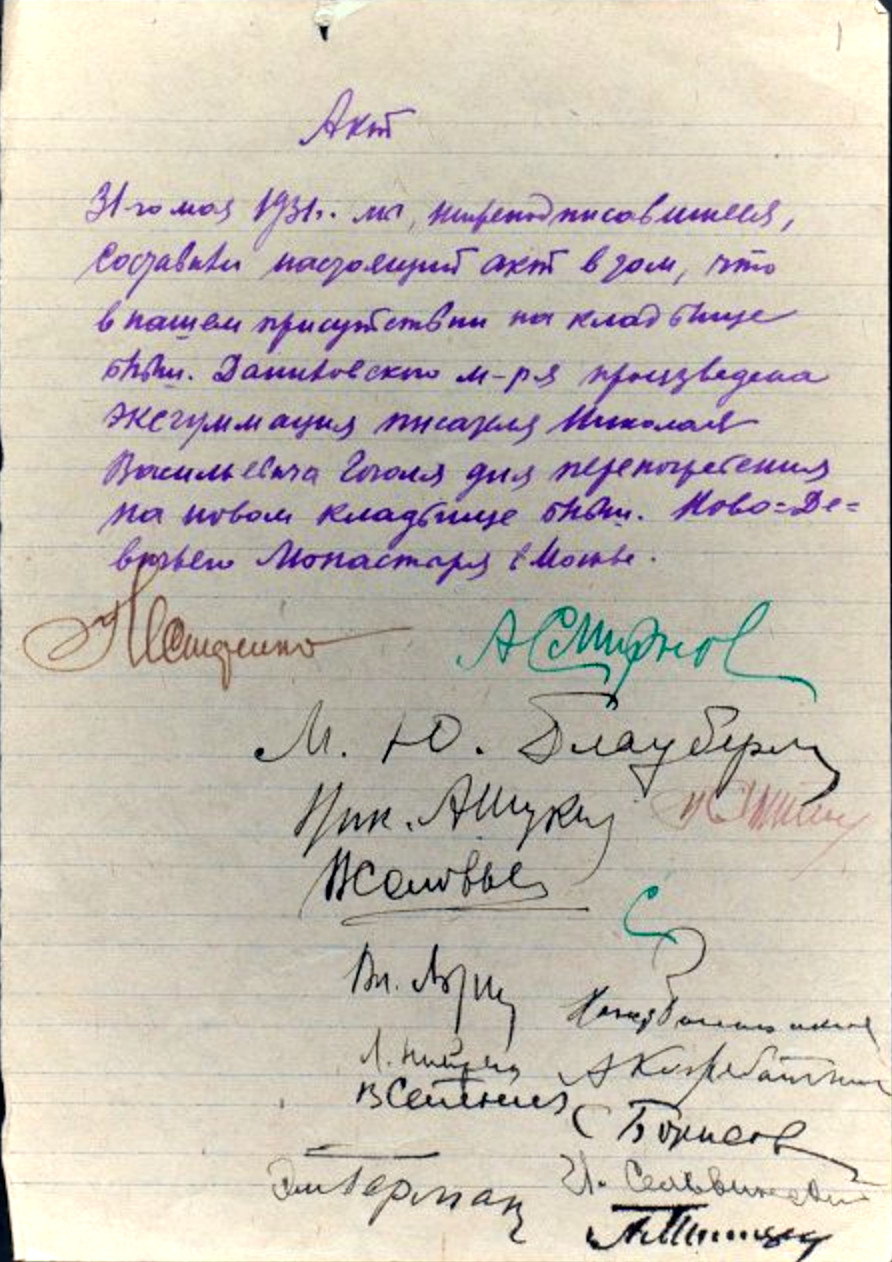
\includegraphics[width=0.95\linewidth]{act-hi-gimp.jpg}\\

\textit{Акт о вскрытии могилы Н. В. Гоголя, 31 мая 1931}
\end{center}

\vspace*{\fill}

\newpage


\begin{center}
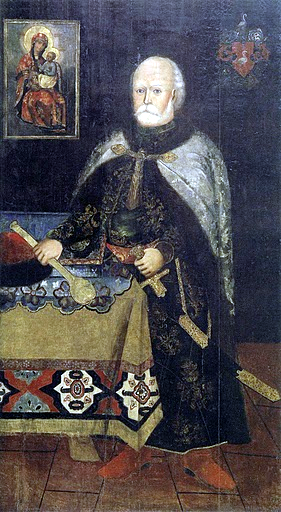
\includegraphics[width=0.85\linewidth]{Vasil-Dunin-Borkovskiy.png}\\

\textit{Василий Дунин-Борковский}
\end{center}



\newpage

%\backmatter

%\appendix
%\addappheadtotoc


%\input{appendix/dict.tex}

\begin{thebibliography}{999}
\bibitem{zeleninrusalki}
\emph{Избранные труды. Очерки русской мифологии: Умершие неестественною смертью и русалки}. Зеленин Д. К. Индрик, Москва, 1995.

\bibitem{kak}
\emph{Как Владимир идолов низвергал}. Петр Семилетов, DOI 10.5281/zenodo.14212537

\bibitem{volos}
\emph{Скотий бог Волос}. Петр Семилетов, DOI 10.5281/zenodo.14563494
\end{thebibliography}


\end{document} 